\documentclass{article}
\usepackage{graphicx}
\usepackage{amsmath}
\usepackage{hyperref}
\usepackage{cite}
\usepackage{listings}
\usepackage{xcolor}
\usepackage{ulem}

\lstset{
    language=R,                  % Specify R as the language
    basicstyle=\ttfamily,        % Use monospaced font for code
    keywordstyle=\color{blue},   % Color for keywords
    commentstyle=\color{gray},   % Color for comments
    stringstyle=\color{red},     % Color for strings
    numbers=left,                % Line numbers on the left
    numberstyle=\tiny\color{gray}, % Style for line numbers
    stepnumber=1,                % Number every line
    frame=single,                % Frame around the code
    breaklines=true              % Enable line breaking
}

\graphicspath{{finalproject/images/}}

\title{Daily Trip Duration Analysis of Uber Rides in NYC Using Time Series Methods }
\author{
    Farooq Mahmud
}

\date{August 7, 2025}

\begin{document}

\maketitle

\section{Introduction}
Urban mobility has undergone a transformative shift with the proliferation of ride-hailing services such as Uber. In dense metropolitan areas such as New York City, these services generate massive amounts of data that can reveal important patterns in travel behavior. This project proposes a time series analysis of average daily Uber trip durations in New York City throughout the year 2024, using publicly available high-volume for-hire vehicle (FHV) trip data.

The data set is sourced from the NYC Taxi and Limousine Commission (TLC) and contains more than 150 million records for 2024 alone. For the purpose of this analysis, a subset of the data has been prepared using PySpark to compute the average duration of Uber trips per day, resulting in 365 data points. The data set is accessible through the NYC TLC portal\cite{nyctlc2024}.

The main objective of this project is to explore the temporal behavior of Uber trip durations and apply time series modeling to understand and forecast future values. Specific goals include examining stationarity, identifying appropriate models through diagnostics, and evaluating the accuracy of forecasts. A review of previous research indicates that ride-hailing data have been used extensively for congestion, demand prediction, and fleet optimization, but less so for temporal duration modeling at a daily resolution.

Two references guiding this work are (1) Tandon et al. (2024), which evaluates the effect of congestion pricing on ride-hailing behavior in New York City\cite{tandon2024congestion} and (2) Ma et al. (2024), which explores congestion-aware scheduling of electric ride-hailing fleets\cite{ma2024congestion}.

This study contributes by applying time series methods to a large-scale, real-world dataset to understand trends and variability in urban travel times.

\section{Preliminary Analysis}

The dataset used in this study consists of the average daily trip duration (in minutes) for Uber trips in New York City throughout 2024. This time series was constructed by aggregating more than 150 million ride records published by the New York Taxi and Limousine Commission. A PySpark pipeline was used to compute the average duration per day, resulting in a time series of 366 observations (one for each day in the leap year 2024).


To begin the exploratory phase, a time series line plot of the daily average trip durations was generated. Figure~\ref{fig:initial_plot} displays this unannotated time series. Several key patterns emerge, even without additional labeling. The plot exhibits moderate variability throughout the year with visible periodic fluctuations. A general upward trend is observed during the summer months, suggesting seasonal effects. There also appear to be isolated spikes and drops, which may correspond to holidays, weather events, or changes in urban mobility behavior.

\begin{figure}
  \centering
  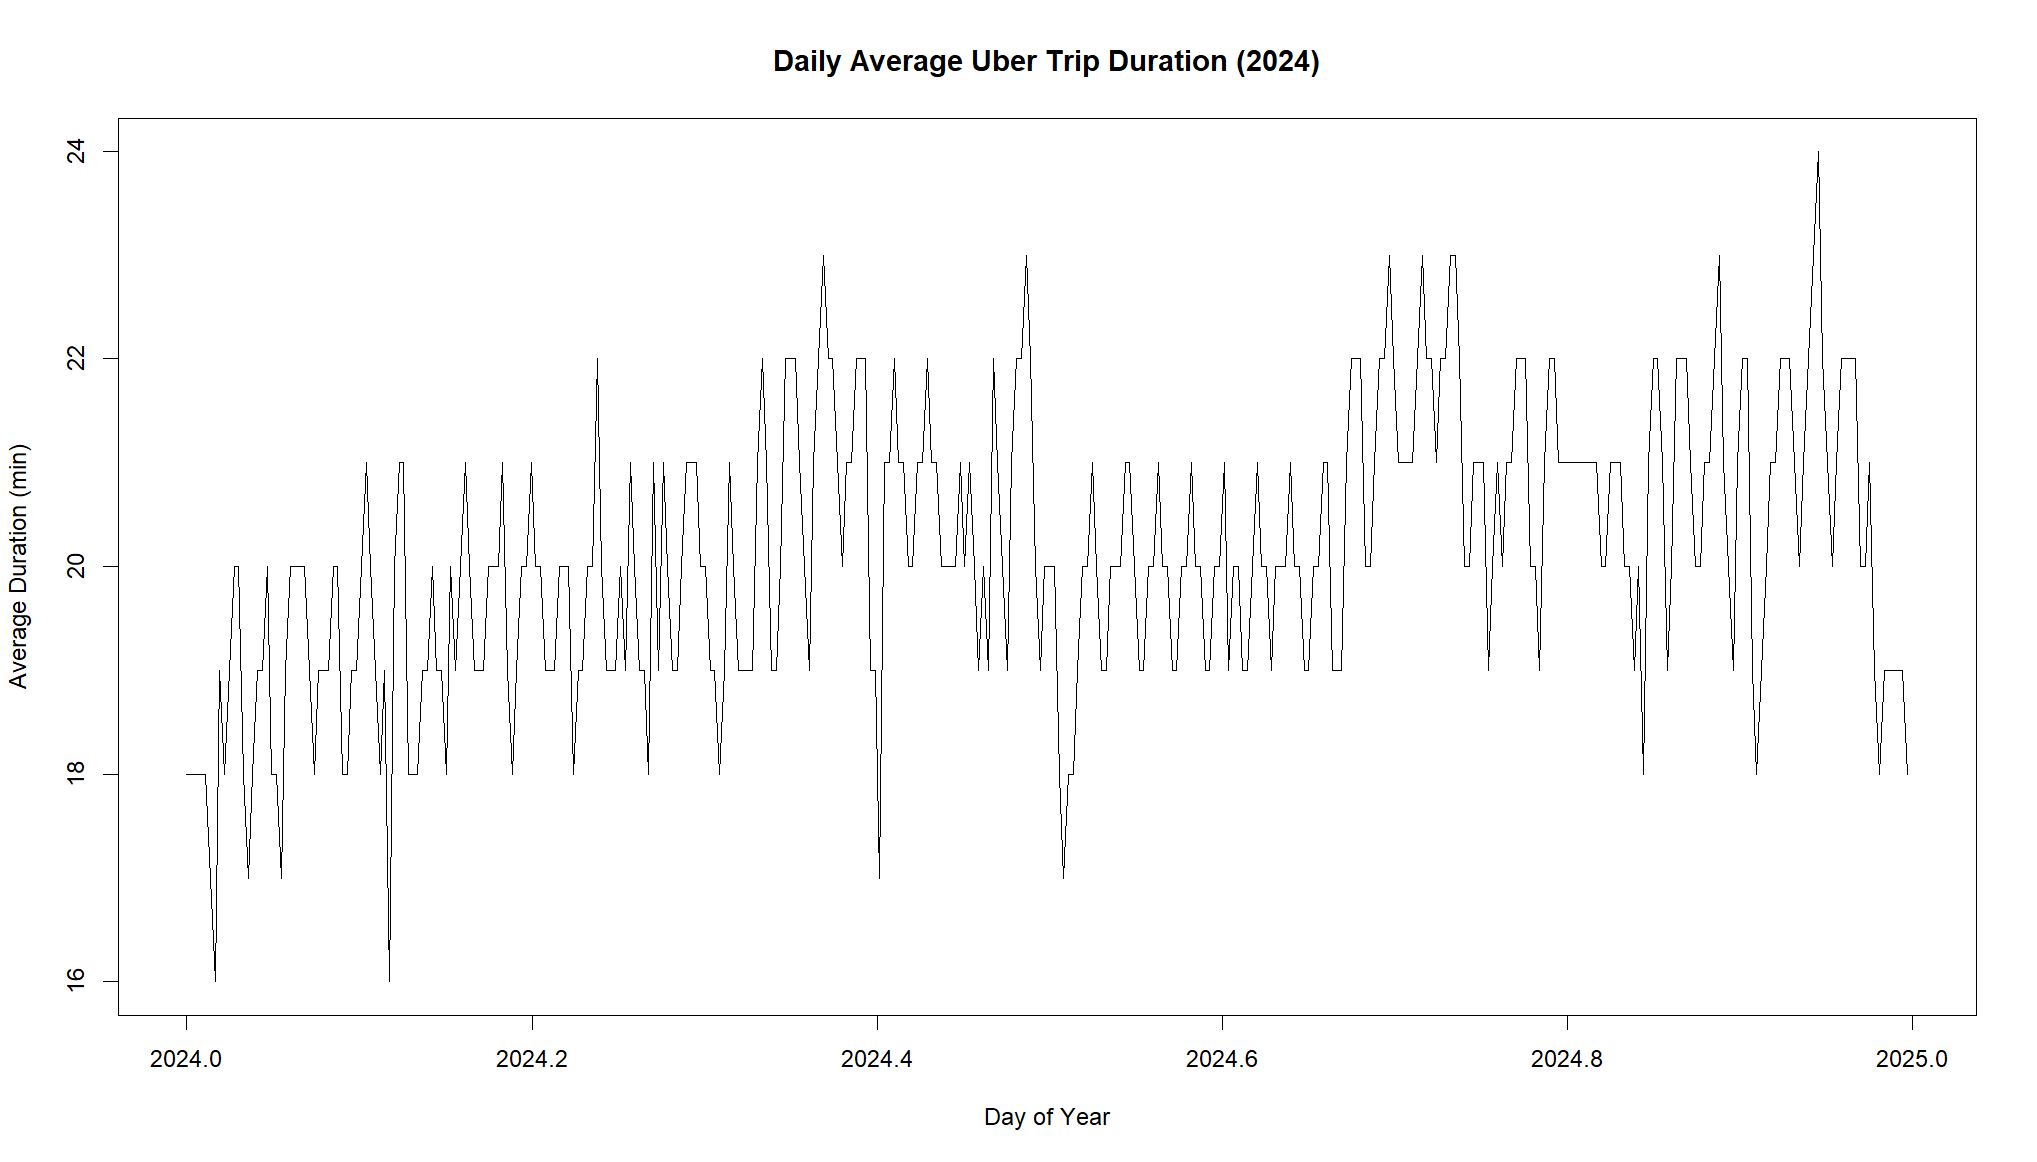
\includegraphics[width=\textwidth]{avg_trip_duration_simple.png}
  \caption{Daily average Uber trip duration in NYC for 2024.}
  \label{fig:initial_plot}
\end{figure}

In an attempt to expose more patterns, a second version of the time series plot was created with Fridays, Saturdays, Sundays, and the major holidays in the United States highlighted (Figure~\ref{fig:timeseries_plot}). This annotated visualization reveals more structured weekly seasonality, with higher average durations occurring more frequently on weekends. Holidays such as Independence Day, Labor Day, and Thanksgiving are associated with pronounced decreases in duration.

\begin{figure}
  \centering
  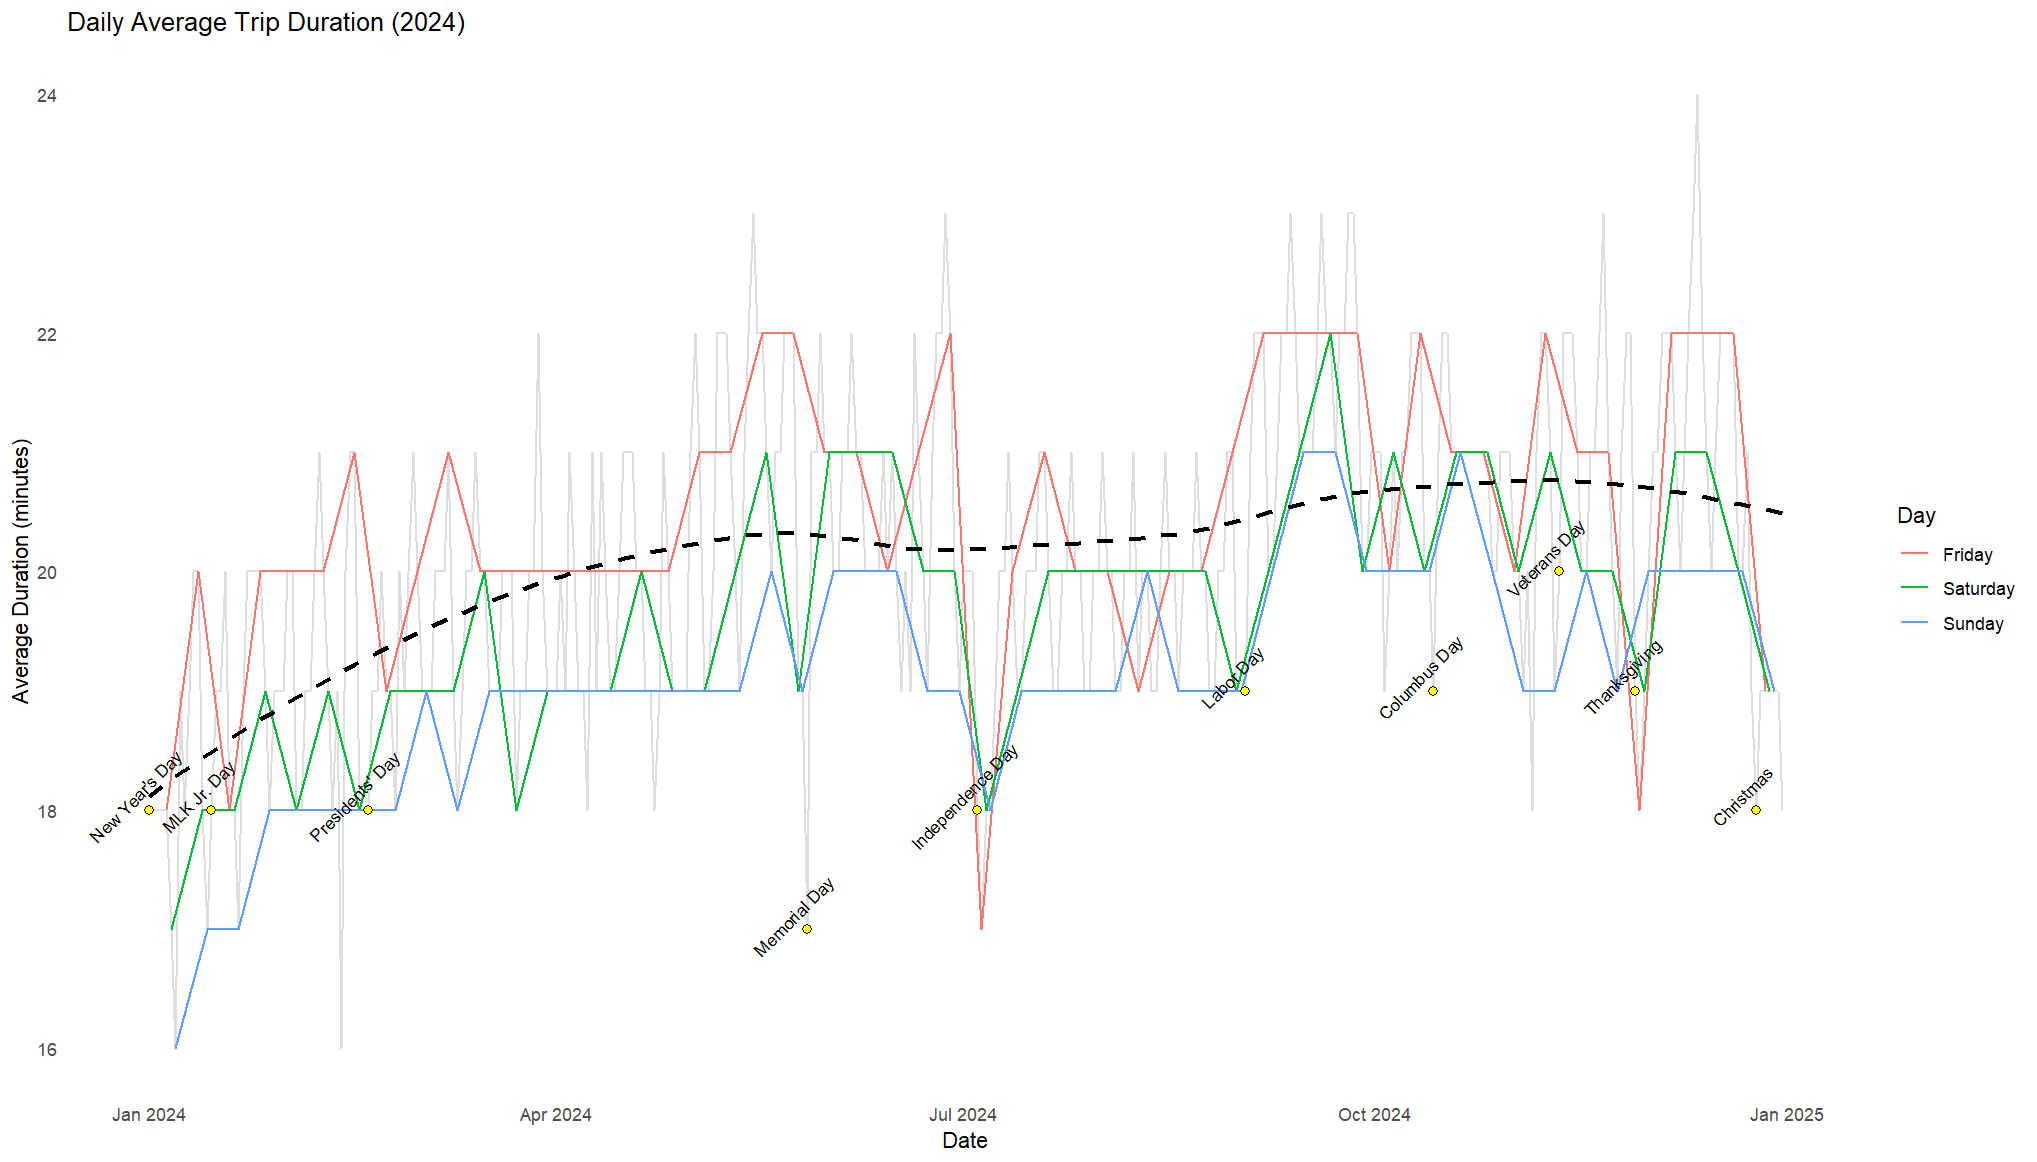
\includegraphics[width=\textwidth]{avg_trip_duration_by_day.png}
  \caption{Daily average Uber trip duration in NYC for 2024, with weekends and holidays highlighted.}
  \label{fig:timeseries_plot}
\end{figure}


To determine whether the daily average Uber trip duration series is stationary, we performed the Augmented Dickey-Fuller (ADF) test. The ADF test yielded the following results:

\begin{quote}
\texttt{Dickey-Fuller = -3.4658, Lag order = 7, p-value = 0.04612}
\end{quote}

Because the p-value is less than 0.05, we reject the null hypothesis at the significance level 5\%. Therefore, there is statistical evidence to suggest that the time series is stationary.

The ACF plot (Figure~\ref{fig:acf_plot}) shows a slow and gradual decline, consistent with a nonstationary series. This pattern suggests the presence of a trend and the need to differentiate the series to induce stationarity. Significant autocorrelation at multiple lags may also indicate latent seasonality.

\begin{figure}
  \centering
  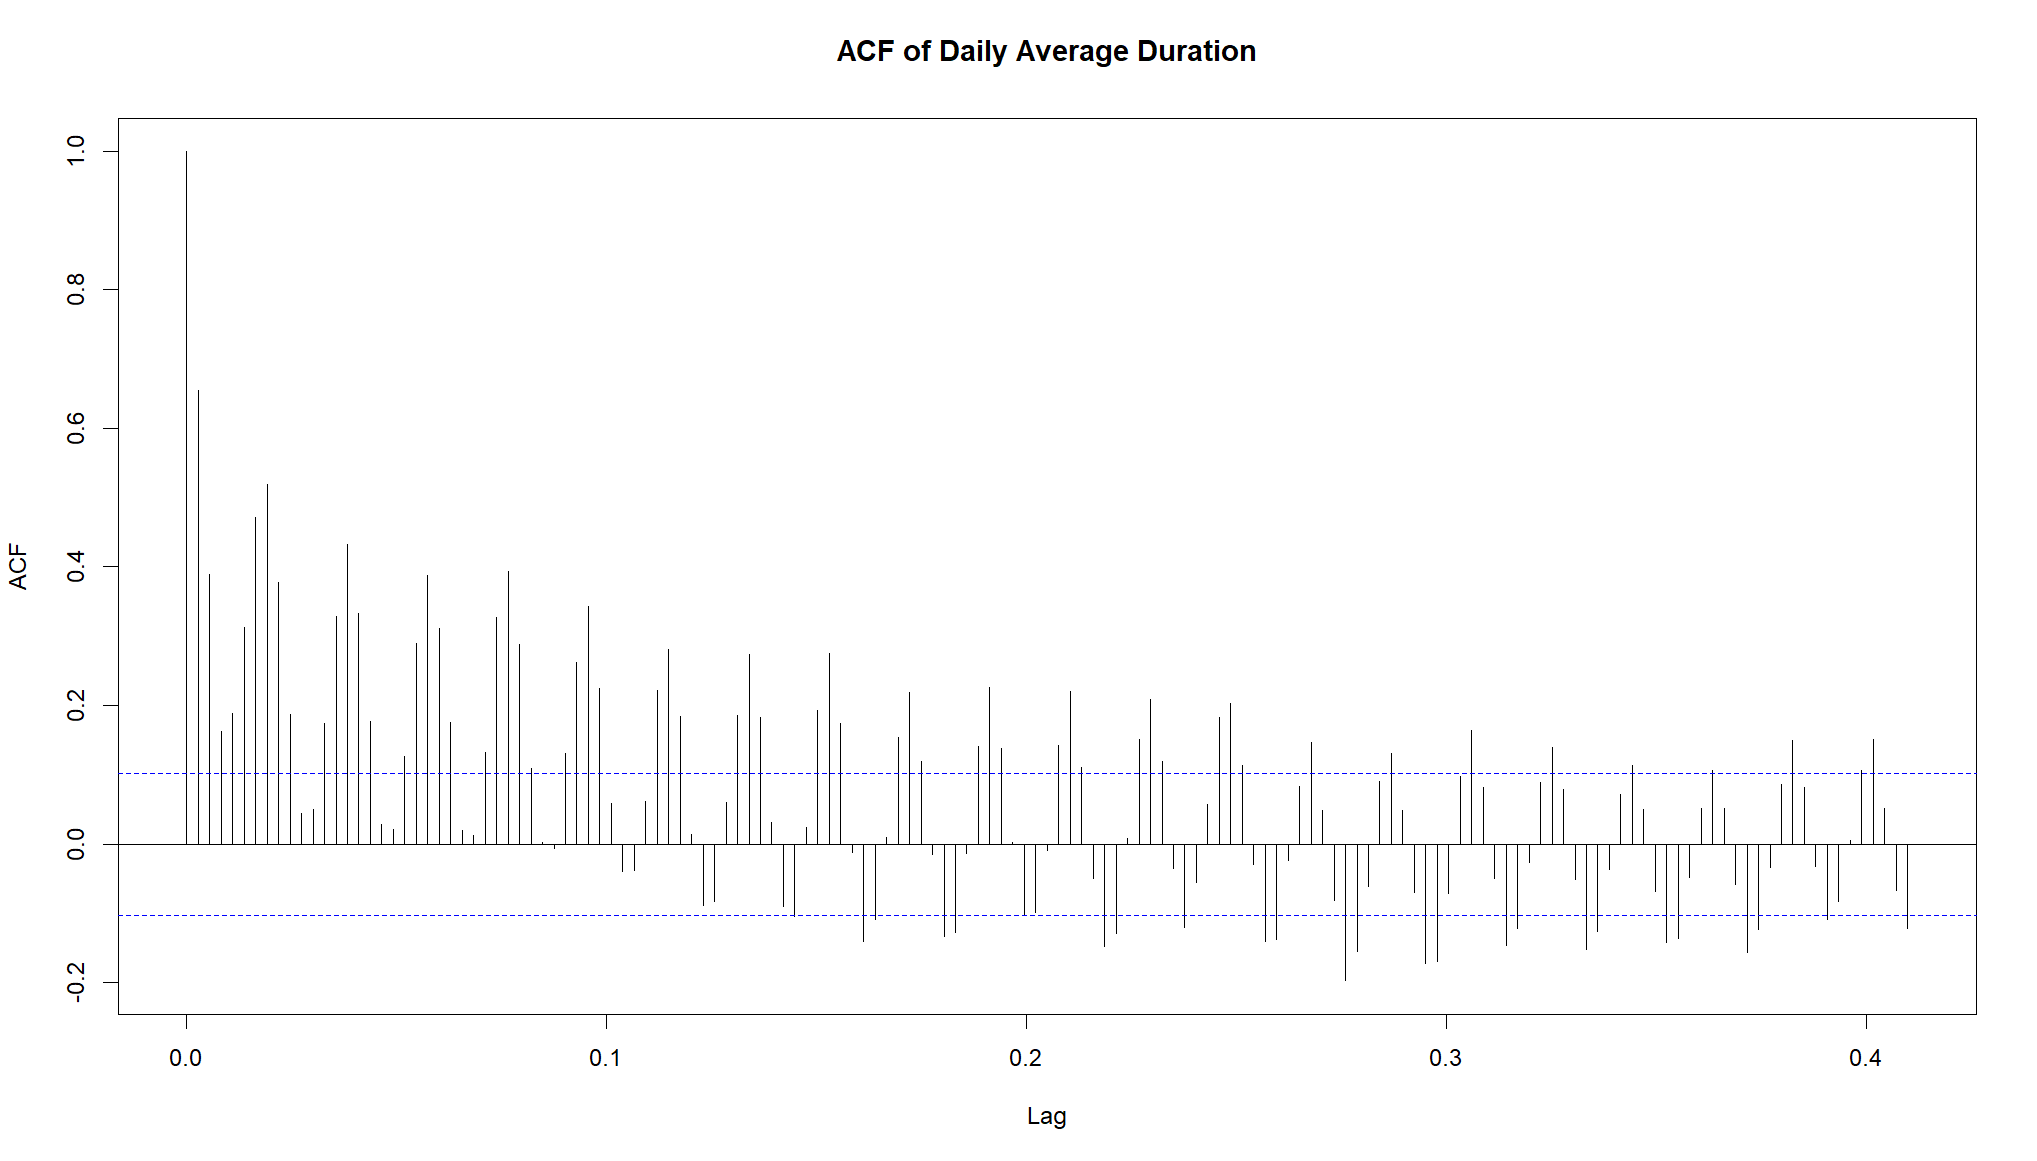
\includegraphics[width=\textwidth]{finalproject/images/acf-plot.png}
  \caption{Autocorrelation Function (ACF) plot of daily average trip durations. The plot shows a slow decay, suggesting non-stationarity and potential seasonality in the data.}
  \label{fig:acf_plot}
\end{figure}


The PACF plot (Figure~\ref{fig:pacf_plot}) shows a large spike at lag 1, followed by a tapering tail of smaller spikes. This pattern suggests the existence of an autoregressive (AR) structure in the series. The combination of these findings supports the consideration of ARIMA modeling, potentially with seasonal differencing.

\begin{figure}
  \centering
  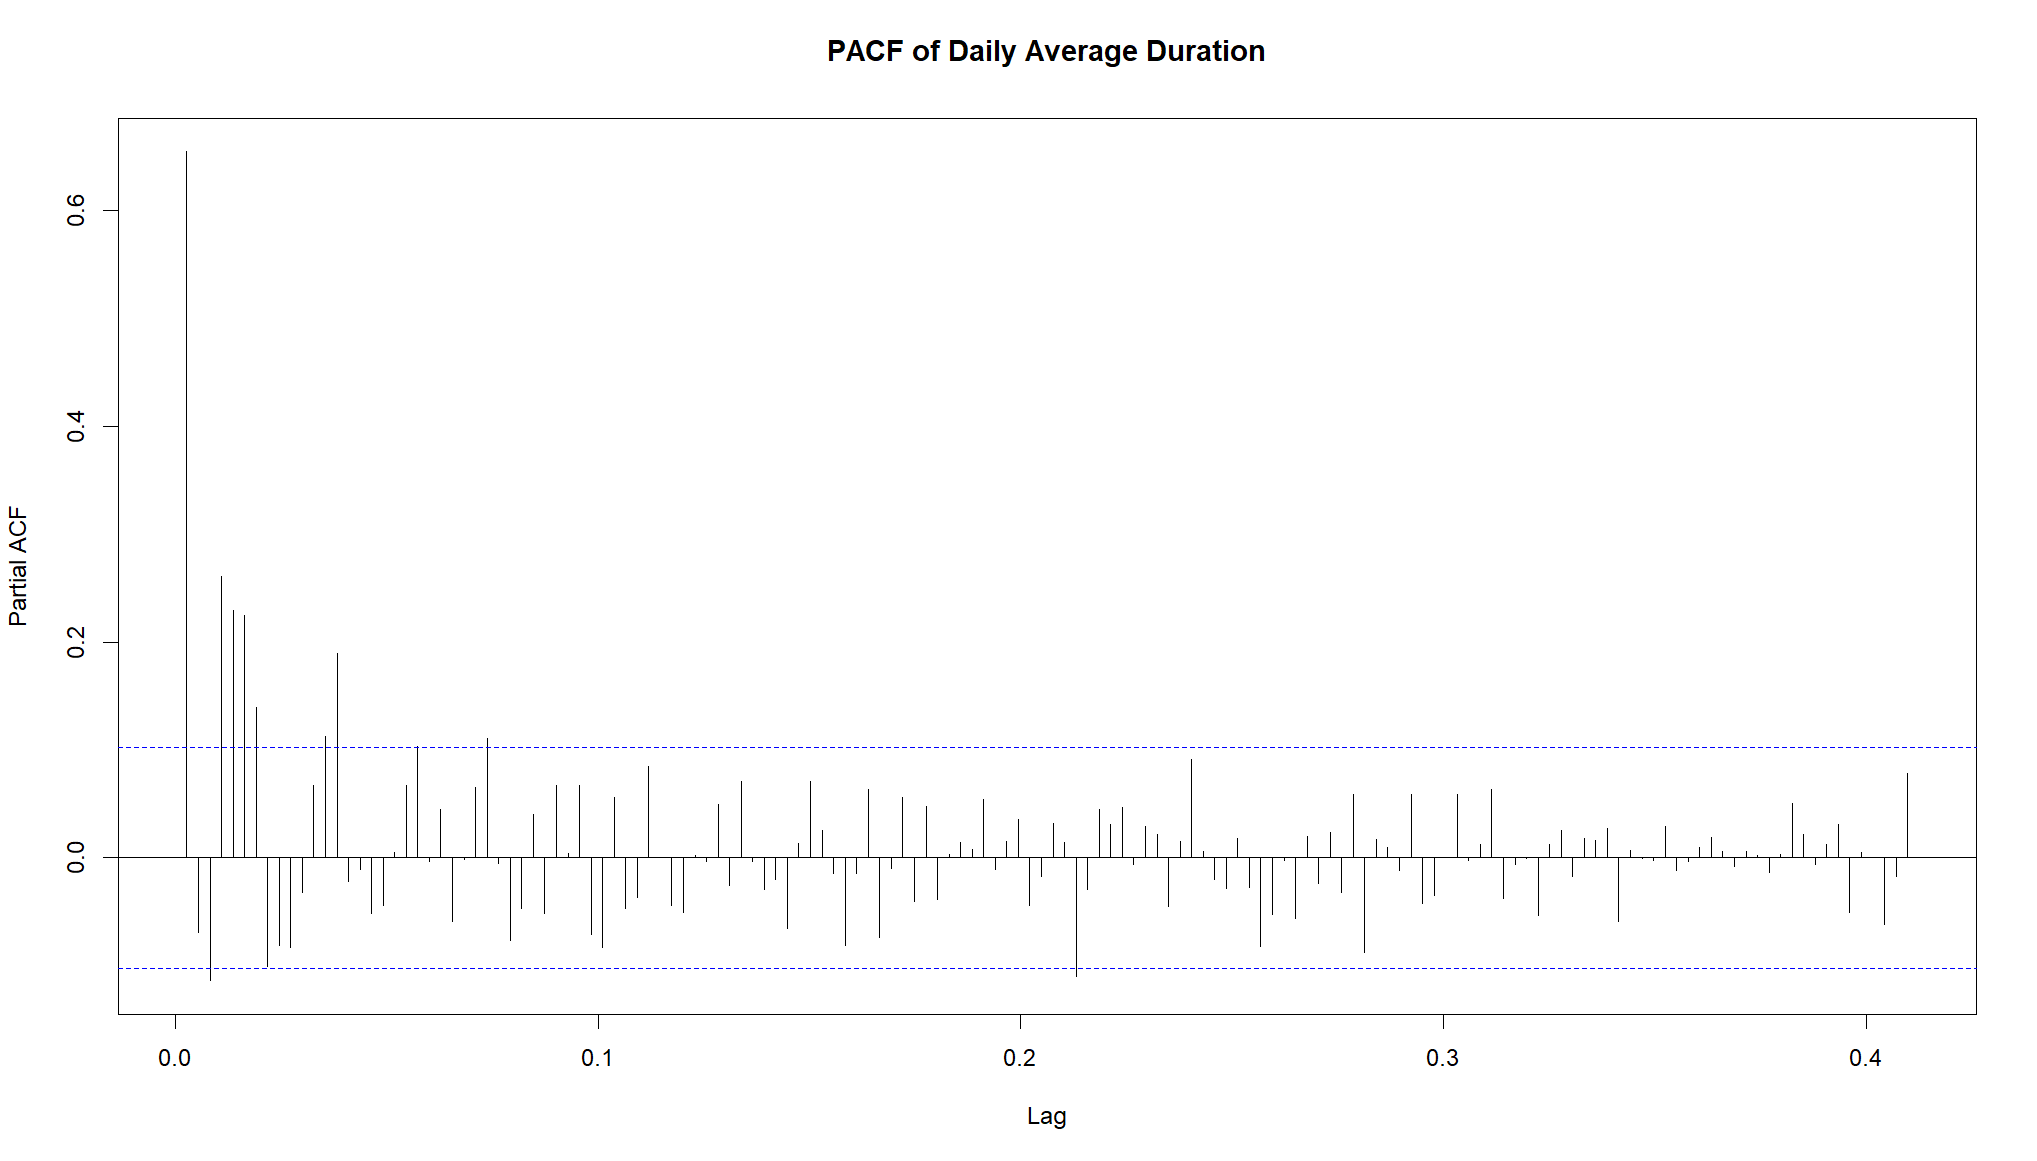
\includegraphics[width=\textwidth]{finalproject/images/pacf-plot.png}
  \caption{Partial Autocorrelation Function (PACF) plot of daily average trip durations. The sharp drop after the first few lags indicates the presence of autoregressive components.}
  \label{fig:pacf_plot}
\end{figure}

Although the ADF test returned a p-value of 0.04612, suggesting stationarity at the 5\% significance level, the ACF and PACF plots exhibit patterns indicative of nonstationarity, including a slow decay in autocorrelation. This discrepancy implies that the series may be only marginally stationary or trend-stationary. To address this, further differencing may be warranted in subsequent model development.

\section {Secondary Analysis}
\section {Discussion and Conclusion}

\bibliographystyle{plain}
\bibliography{finalproject/docs/refs}

\end{document}
